\section{Results}
\label{sec:results}
% FILL: every XX below is finalized from p1_forced_choice.csv (v4),
% p4a_sweep.csv, p4b_*_sweep.csv, p4c_*_sweep.csv, p4e_sweep.csv.

\subsection{Susceptibility: gloss rejected, clones at chance}
\label{sec:res-probe}
The forced-choice probe confronts each agent with one gold product and one
synthetic listing (300 randomized duels). Agents overall still prefer the
real product, $\sigma=\textbf{XX}$ (95\% CI $[\textbf{XX},\textbf{XX}]$,
binomial vs.\ $\tfrac12$ $p=\textbf{XX}$), but the families separate sharply:
$\sigma_{\text{clone}}=\textbf{XX}$ --- indistinguishable from chance
--- while $\sigma_{\text{geo}}=\textbf{XX}$ and
$\sigma_{\text{reviews}}=\textbf{XX}$. Trajectory inspection shows the
mechanism: agents quote instruction attributes, find them missing or altered
on gloss pages, and buy the real product even when it displays no rating and
the synthetic page shows 4.7 stars with thousands of reviews. Social proof
has essentially no pull; specification grounding dominates --- and clones
are the one family engineered to pass specification grounding while failing
the instruction's critical attributes.

\subsection{Dose--response: success flat, regret and confidence climb}
\label{sec:res-dose}
Figure~\ref{fig:dose} and Table~\ref{tab:dose} give the main curve over
$\varepsilon\in\{0,0.1,0.25,0.5,0.75\}$ ($N{=}\textbf{XX}$ tasks per dose,
plus a second-seed replication at the endpoints, $N{=}\textbf{XX}$ paired
observations). Three co-movements define the silent-erosion signature.
\textbf{Success appears tolerable}: from
$\textbf{XX}$ at $\varepsilon=0$ to $\textbf{XX}$ at $\varepsilon=0.75$
(McNemar $\textbf{XX}$). \textbf{Regret climbs steadily}: mean regret
$\textbf{XX}\to\textbf{XX}$ (+\textbf{XX\%}), with the paired endpoint
difference $\textbf{XX}$ (bootstrap 95\% CI $[\textbf{XX},\textbf{XX}]$).
\textbf{Confidence rises}: post-hoc verbalized confidence increases from
$\textbf{XX}$ to $\textbf{XX}$ as contamination grows --- agents err more
while trusting themselves more. The purchase share tells the mechanism
directly: synthetic listings are bought in \textbf{XX\%} of tasks at
$\varepsilon=0.25$ and \textbf{XX\%} at $\varepsilon=0.75$ (from 0\% at
$\varepsilon=0$; Cochran--Armitage trend $p=\textbf{XX}$), and purchases of
synthetic listings carry mean reward $\textbf{XX}$ versus $\textbf{XX}$ for
purchases of real listings at the same dose.

\begin{table}[t]
\centering
\small
\caption{Dose--response of agent decision quality under ambient
contamination (Qwen2.5-7B backbone, mix contamination). XX = finalized from
P4 outputs.}
\label{tab:dose}
\begin{tabular}{lccccc}
\toprule
$\varepsilon$ & Success & S@0.8 & Regret & Synth.\ bought & Conf. \\
\midrule
0.00 & XX & XX & XX & 0\% & XX \\
0.10 & XX & XX & XX & XX\% & XX \\
0.25 & XX & XX & XX & XX\% & XX \\
0.50 & XX & XX & XX & XX\% & XX \\
0.75 & XX & XX & XX & XX\% & XX \\
\bottomrule
\end{tabular}
\end{table}

\begin{figure}[t]
\centering
% 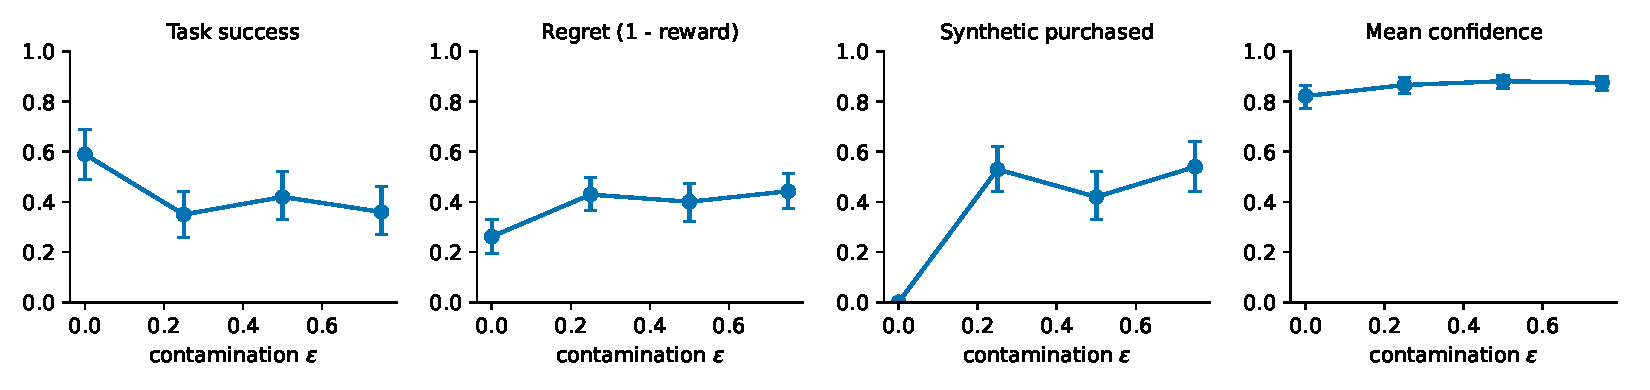
\includegraphics[width=\linewidth]{figures/dose_response.pdf}
\caption{Dose--response under ambient contamination: success, regret,
synthetic-purchase share, and mean confidence as functions of the
contamination level $\varepsilon$ (mix families; $N$=XX tasks per dose;
error bars = 95\% cluster-bootstrap CIs over tasks).}
\label{fig:dose}
\end{figure}

\subsection{Family attribution}
\label{sec:res-family}
Single-family runs at $\varepsilon=0.75$ (Table~\ref{tab:family}) attribute
the damage. Clone contamination is the most destructive
(success $\textbf{XX}\to\textbf{XX}$; regret $+\textbf{XX\%}$), consistent
with the probe; geo and reviews are milder, with geo essentially invisible
at the success level yet still taxing regret by \textbf{XX\%} ---
quiet attrition rather than collapse.

\begin{table}[t]
\centering
\small
\caption{Per-family contamination at $\varepsilon=0.75$ (40 paired tasks).
XX = finalized from P4B outputs.}
\label{tab:family}
\begin{tabular}{lcccc}
\toprule
Family & Success$_0$ & Success$_{.75}$ & Regret$_0$ & Regret$_{.75}$ \\
\midrule
geo & XX & XX & XX & XX \\
clone & XX & XX & XX & XX \\
reviews & XX & XX & XX & XX \\
\bottomrule
\end{tabular}
\end{table}

\subsection{Defenses: provenance beats detection}
\label{sec:res-defense}
Table~\ref{tab:defense} evaluates the defense battery at
$\varepsilon=0.75$ against the paired uncontaminated baseline.
Provenance re-ranking recovers \textbf{XX\%} of the incurred regret
(oracle: \textbf{XX\%}), while the matched random filter recovers only
\textbf{XX\%} --- filtering \emph{quality}, not filtering \emph{amount},
does the work. The perplexity detector, calibrated to near-perfect
separation on a held-out sample (real pages: 15--167 perplexity; synthetic:
7--22), recovers \textbf{XX\%}; the structural detector \textbf{XX\%}; the
prompt defense \textbf{XX\%}. Detection helps on gloss-heavy families and
fails on clones --- exactly where provenance, which does not inspect
content, still works.

\begin{table}[t]
\centering
\small
\caption{Defense battery at $\varepsilon=0.75$ (mix contamination, 40 paired
tasks). Recovery = fraction of incurred regret (vs.\ $\varepsilon=0$)
eliminated. XX = finalized from P4C outputs.}
\label{tab:defense}
\begin{tabular}{lccc}
\toprule
Defense & Success & Regret & Recovery \\
\midrule
none (high dose) & XX & XX & 0\% \\
random (matched drop) & XX & XX & XX\% \\
prompt & XX & XX & XX\% \\
detector-struct & XX & XX & XX\% \\
detector-text (ppl) & XX & XX & XX\% \\
provenance (noisy bit) & XX & XX & XX\% \\
oracle (upper bound) & XX & XX & XX\% \\
\bottomrule
\end{tabular}
\end{table}

\subsection{Backbone generality and scale}
\label{sec:res-backbone}
The dose--response replicates on Llama-3.1-8B
(success $\textbf{XX}\to\textbf{XX}$; regret $\textbf{XX}\to\textbf{XX}$),
and scale ablations at $\varepsilon=0.75$ with Qwen2.5-3B/1.5B show
\textbf{XX} --- smaller agents are \emph{more} susceptible, so the
vulnerability is not an artifact of one model's quirks.
